\documentclass[tikz,border=2pt]{standalone}
\renewcommand{\familydefault}{\sfdefault}
\usetikzlibrary{arrows.meta,calc,positioning}
\tikzset{every picture/.style={line width=1pt, >=Stealth},
         hl/.style={fill=black, fill opacity=0.12, text opacity=1}}
\usetikzlibrary{decorations.pathreplacing}
\begin{document}
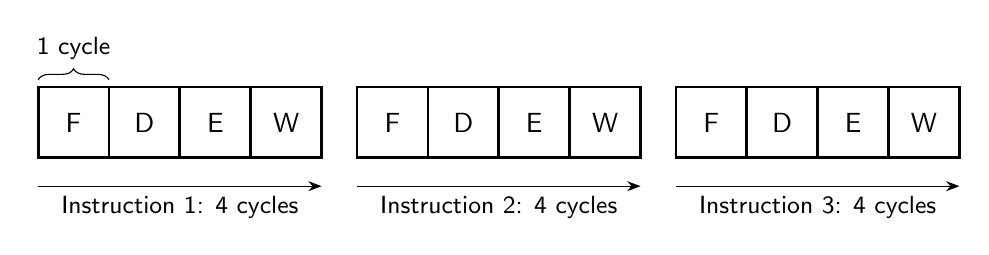
\begin{tikzpicture}[x=0.9cm, y=0.9cm, cell/.style={draw, minimum size=0.9cm}]
  % \pipe{row}{first cycle}{stage/style, ...}: one instruction, one cell per clock cycle
  \newcommand{\pipe}[3]{\foreach \v/\s [count=\i from 0] in {#3} \node[cell, \s] at (#2 + \i, -#1) {\v};}
  % Without pipelining, each instruction runs all four stages before the next one starts.
  \foreach \k in {0, 1, 2} {
    \pipe{0}{4.5*\k}{F/, D/, E/, W/}
    \draw[->, thin] (4.5*\k - 0.5, -0.9) -- node[below, font=\small] {Instruction \the\numexpr\k+1\relax: 4 cycles} (4.5*\k + 3.5, -0.9);
  }
  \draw[decorate, decoration={brace, amplitude=4pt}, thin] (-0.5, 0.6) -- node[above=4pt, font=\small] {1 cycle} (0.5, 0.6);
\end{tikzpicture}
\end{document}
